\chapter{Introduction}
\section{But why}
\section{Requirement engineering}
In a complex system, there are many stakeholders, both internal and external.
The requirements are meant to capture the needs of the users and convey them to
the developers~\cite{ibm_req}. It is important that the requirements are
unambiguous~\cite{ibm_req, rupp2014}. Since natural language is ambiguous by
nature, there are frameworks and templates to improve the quality of the
requirements~\cite{rupp2014}. 

\subsection{User and system requirements}
Requirements can be organized into two categories, User and System requirements.
These differ in a number of ways, both in their nature and how they are
procured.

A project design starts with a need from a customer or user. These needs set the
goal of the project and are of a high level, abstract nature. They are captured
from the future users of the system and are expressed in the users language. In
essence, the User requirements describe the problem that is to be solved by the
system~\cite{ibm_req}. 

When the User requirements are set, they need to be condensed into technical
requirements that the developers can work towards. These are the System
requirements. They define what the system and its sub-systems do. It is the
developers that own these requirements and they are responsible that these in
turn fulfill the User requirements~\cite{ibm_req}.

\subsection{Requirement formulation}
It is important that requirements are clear and unambiguous. By using templates
when expressing the requirements, there is a framework where it is agreed what a
word/phrase means. This greatly increases the quality of the requirements
\cite{rupp2014}. By using a template for the structure of a requirement, it is
ensured that all parts needed are in the requirement. Rupp~\cite{rupp2014}
gives a template on how to formulate a requirement~\ref{fig:req_template}.
\begin{figure}[H]
    \centering
    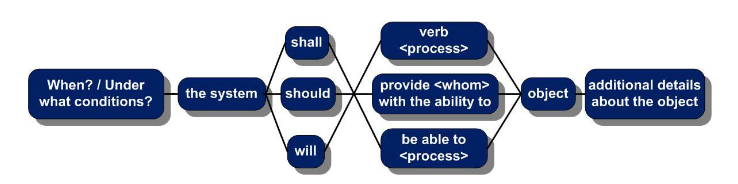
\includegraphics[width=\textwidth]{./img/introduction_req_template.PNG}\label{fig:req_template}
    \caption{Requirement formulation template.}
\end{figure}
\subsection{Requirement software}
In a complex system, there are many relationships between stakeholders and
requirements~\cite{ibm_req}. A change in one requirement may affect several other
requirements. Therefore, it is important to have a requirement software that
makes it easy to track the dependencies between the different requirements.

% More info on requirement system 


\section{Shell Eco-Marathon}
Shell Eco-Marathon (TODO ref to webpage) is a yearly competition for students to compete with fuel efficient, custom made, vehicles.

There are two main class divisions, ´´Prototype'' and ´´Urban Concept
Vehicle''. There are also sub classes based on fuel/energy type, with a range
of fuels to chose from. Each fuel has an assigned energy value (TODO ref to
rules) which makes different fuel types comparable. 

\subsection{London Track}
All vehicles drive the same amount of laps, 8 in 2016 (TODO ref to rules), which equals TODO kilometers. Compared to earlier tracks the London track has a steeper height profile. To clime the steepest part of the track the vehicles must deliver larger amounts of torque than might have been used earlier years (this is true for Elba). 

\subsection{Inspections}
Before any vehicle is allowed on the track it must first pass two inspections, the safety inspection covers issues related to the safety of the driver and personnel and surrounding cars. 

The technical inspection covers the vehicle compliance to the rules, specifically energy usage. This ensures that the car does not use power from the auxiliary power-source to propel the vehicle in any way.

Simply passing these inspections is the main goal for many of the teams attending SEM (if the car does not change it is simpler to make the car race the next year TODO fix engrish).
